\section{System Designs}
In this section, all of the design aspects of this system have been detailed and justified. This includes the design of the user interface itself, the navigation and expected user path through the application, and the internal design of the application.

\subsection{Navigation/Control Flow Design}
In the final implementation of the system, there were seven main sections, which have been enumerated below with a brief explanation of what their main purpose is.

\begin{enumerate}
	\item Route Discovery \ \\
	The landing page, which provides a large search box (allowing users to search for routes), and a description of the main functionality of the website.
	\item Route Listing \ \\
	The search results page, which would list all of the results returned for a particular set of search terms, as well as some brief information about each of the routes.
	\item Route Detail\ \\
	The individual route display page, which lists all the available information for a given route, as well as the social stream that users can interact with.
	\item Route Creation\ \\
	The map interface that allows users to specify their own routes, as well as a interface for listing the points on the route.
	\item Profile Page\ \\
	The user detail page, which allows registered users to view their own routes and their saved routes, edit their settings, and update their avatars appearance.
	\item Admin Page\ \\
	The administrator only page which gives them access to various administrative tools, as well as the ability to look at and handle reported content.
	\item Login/Signup Pages\ \\
	Pages that provided short forms allowing users to either sign up or log in to the system.
\end{enumerate}
\noindent 
When designing a website, it's important to think about how the users of that website will traverse it, depending on their goals. For Niceway.to, there are two main user groups to consider: those with accounts, and those without accounts. Both of these groups will use the site in very different ways: those users without accounts will use the site simply for the searching of routes, but those \emph{with} accounts will be much more involved in the social aspects of the site and sharing their own content.\ \\
\ \\
The path that users \emph{without} accounts would usually take, as shown in figure \ref{fig:nonuser_flow}, would start with the landing page. They would then follow a rather linear path through the system, as they are only given the choice to advance to the next page in the sequence (or back if they so wish). This starts with searching for a route, selecting a route from the search results, viewing this routes detail page, and then potentially looking at the route in ``full-view'' (where we see the route displayed in a map filling the entire screen). At any point in this sequence, the user is free to jump to the sign up page, a link to which is located in the top right hand corner of every page.

\begin{figure}[!ht]
	\begin{center}
		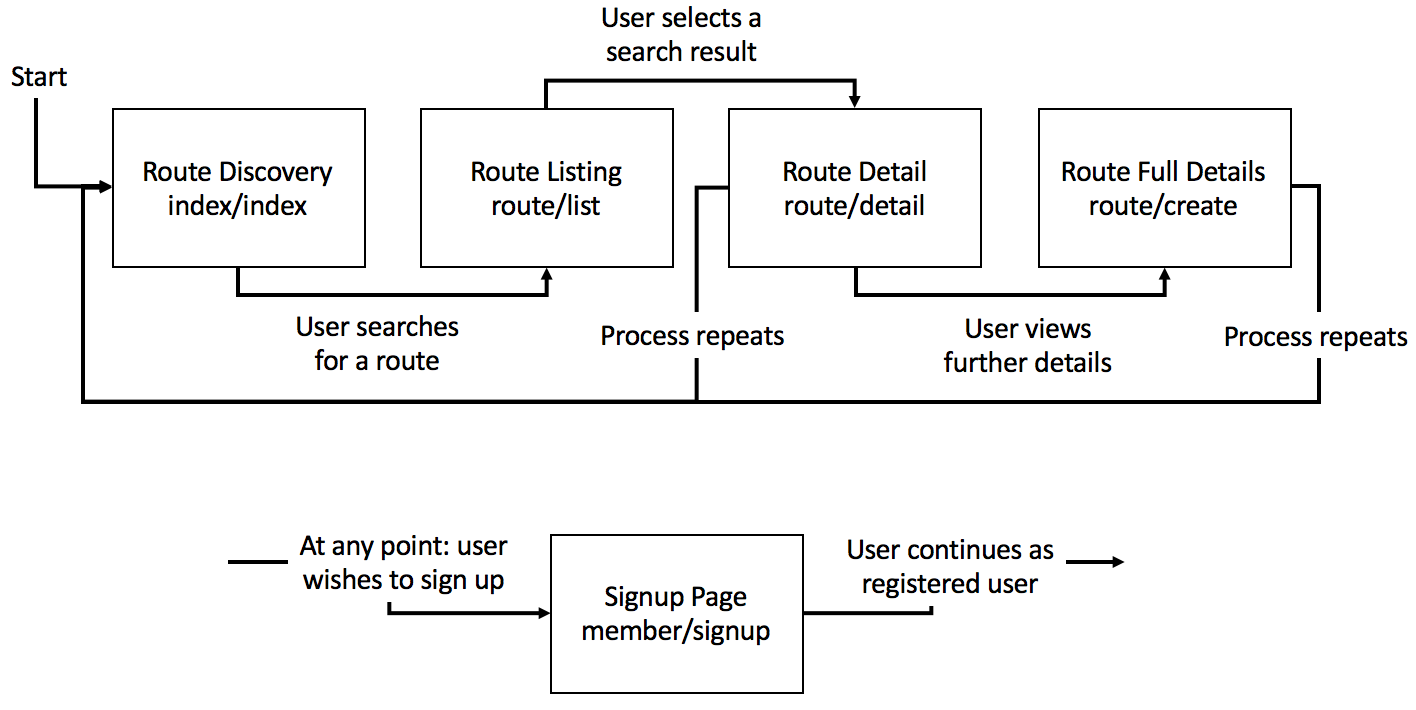
\includegraphics[width=0.9\textwidth]{images/design/nonuser_flow.png}
	\end{center}
	\vspace{-6mm}
	\caption{Expected path of non-registered users}
	\label{fig:nonuser_flow}
\end{figure}

\noindent 
For a registered user, we can expected a much less linear path, due to the larger quantity of actions they have available to them, this path is shown in figure \ref{fig:user_flow}. Unlike the non-registered users, there's no requirement for these users to start on the landing page, as it can be assumed that they would have book marked specific pages, and would need to log in to access them. After logging in, it is expected the user would spend some time on their profile page, and then using this page as the springboard into one of three main actions: looking at their own routes or routes they are interested in, creating a new route, or following the same route search flow as non-users would.

\begin{figure}[!ht]
	\vspace{-5mm}
	\begin{center}
		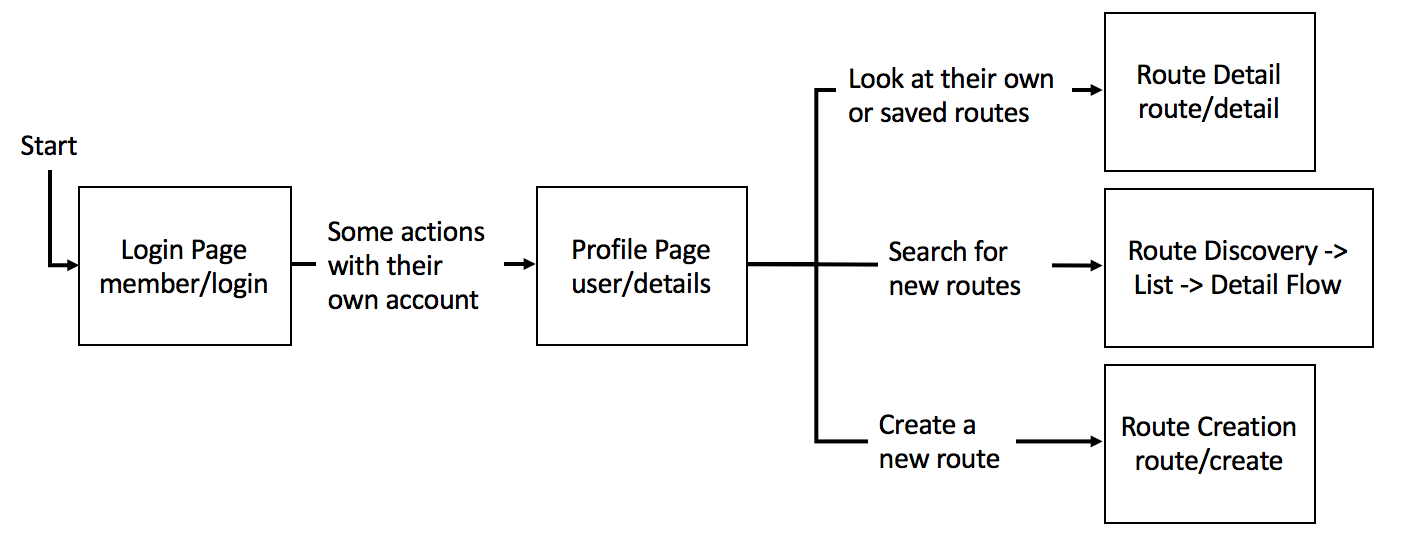
\includegraphics[width=0.9\textwidth]{images/design/user_flow.png}
	\end{center}
	\vspace{-6mm}
	\caption{Expected path of registered users}
	\label{fig:user_flow}
\end{figure}

\noindent
Of course, this is just the generally expected path, and users are in no way restricted to what they can do (with the acceptable of accessing the search results page without having performed a search). The user can access any page of the site from any other page, through use of the navigation bar present on every page (shown in figure \ref{fig:navbar}), which provides links to the search, creation, profile, and administrator sections of the website. This navigation helps to promote freedom and a sense of control within the system. This means that even when users make mistakes, they should feel like they know how to go back and rectify these mistakes, rather than being stuck in a state they do not wish to be in.

\begin{figure}[!ht]
	\begin{center}
		
\includegraphics[width=0.9\textwidth]{images/design/navbar.png}
	\end{center}
	\vspace{-6mm}
	\caption{The navigation bar displayed to registered users}
	\label{fig:navbar}
\end{figure}

\subsection{User Interface Design}
In this section, the interface for each of the main pages of the application have been displayed, along with justifications for why they were designed the way they were. Designed for each of these pages were produced at the beginning of the project and shared with the client. The design presents here are based on his feedback, and a combination of the best features from all the other designs. The initial designs can be found in appendix \ref{sec:isd}.

\paragraph{Route Discovery Page/Landing Page}\ \\

\begin{figure}[!ht]
	\vspace{-6mm}
	\begin{center}
		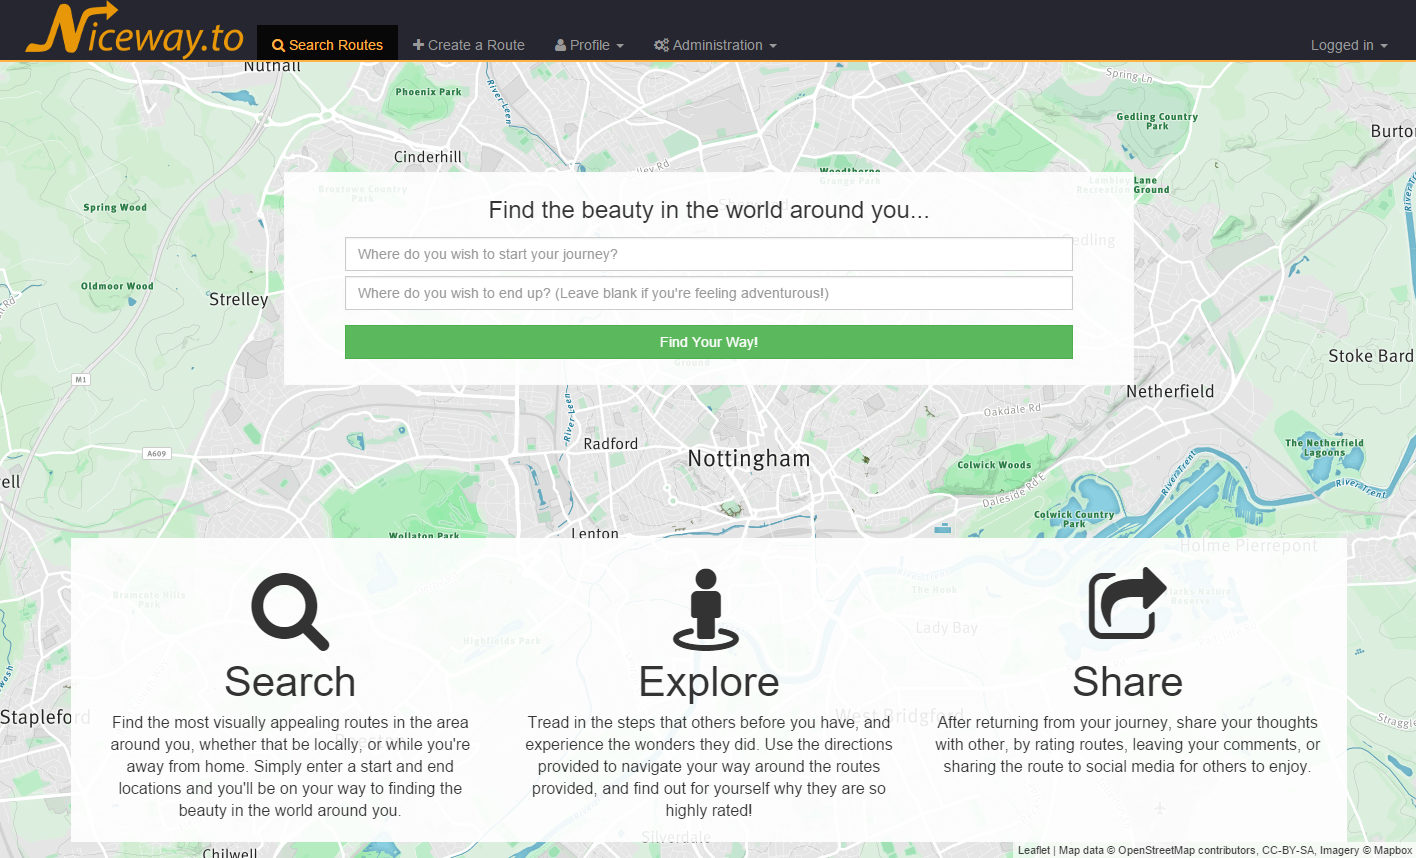
\includegraphics[width=0.95\textwidth]{images/design/landing.png}
	\end{center}
	\vspace{-7mm}
\end{figure}
\noindent 
The design of the landing page was as simple as possible, with a large search box in the centre of the page (similar to Google's website), and a small infographic describing the purpose of the website. The prominent search box promotes the main functionality of the website, and makes it extremely easy for users to get started on their journey, without them being distracted by superfluous extra details. The page aims to look attractive to the user, so they are more compelled to use the site, rather than being put off, and taking their interest elsewhere.

\paragraph{Route Listing Page}\ \\

\begin{figure}[!ht]
	\vspace{-5mm}
	\begin{center}
		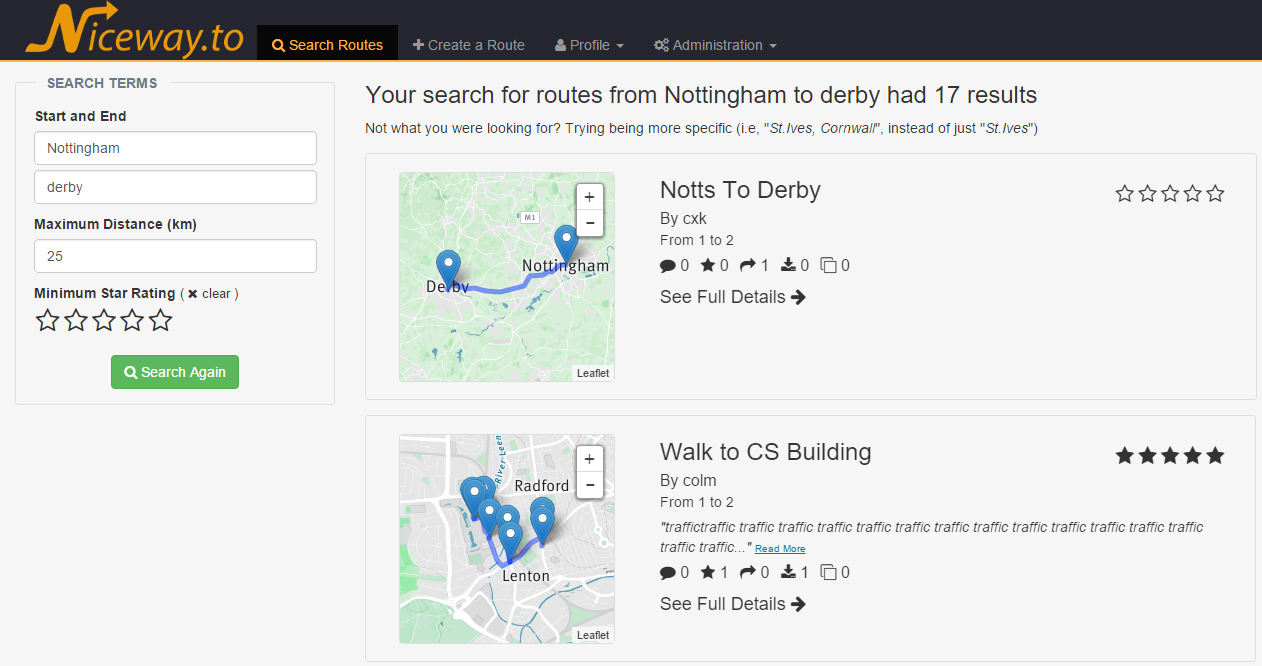
\includegraphics[width=0.95\textwidth]{images/design/listing.png}
	\end{center}
	\vspace{-10mm}
\end{figure}
\newpage 


\noindent 
The route listing page was used to describe the key details of the routes that matched the user's search terms. During the design stage, two main approaches were considered: displaying the routes on a map, or displaying them individually. The problem with the former approach would be when there were a large number of results returned, which would cause the map to look cluttered, and it would be difficult for user to distinguish between routes. The listing approach allows each route to be considered individually, as well as being put in some kind of order (which is where the rating system is utilised). \ \\
\ \\
A form on the left hand side (as well as the large title next to it) is present so that users can see the terms they searched for, and make any amendments necessary if there were mistakes (it is placed on the left because western cultures are more likely to look at the top left of a page first\cite{mccarthy2004could}, which allows users to identify their errors earlier). It also allows them to further refine their search, with a minimum star rating, and maximum distance from the entered points. The key points of each route are displayed on this page, so users can make a decision as to which ones they which to investigate further. This includes the name and description, as well as social ranking, such as the rating, number of social interactions and a summary of comments made on that route. The idea being that a user should very quickly be able to decide if a route is worth visiting or not, so they do not find they are wasting their time looking at poor quality routes.

\paragraph{Route Detail Page}\ \\
\begin{figure}[!ht]
	\vspace{-6mm}
	\begin{center}
		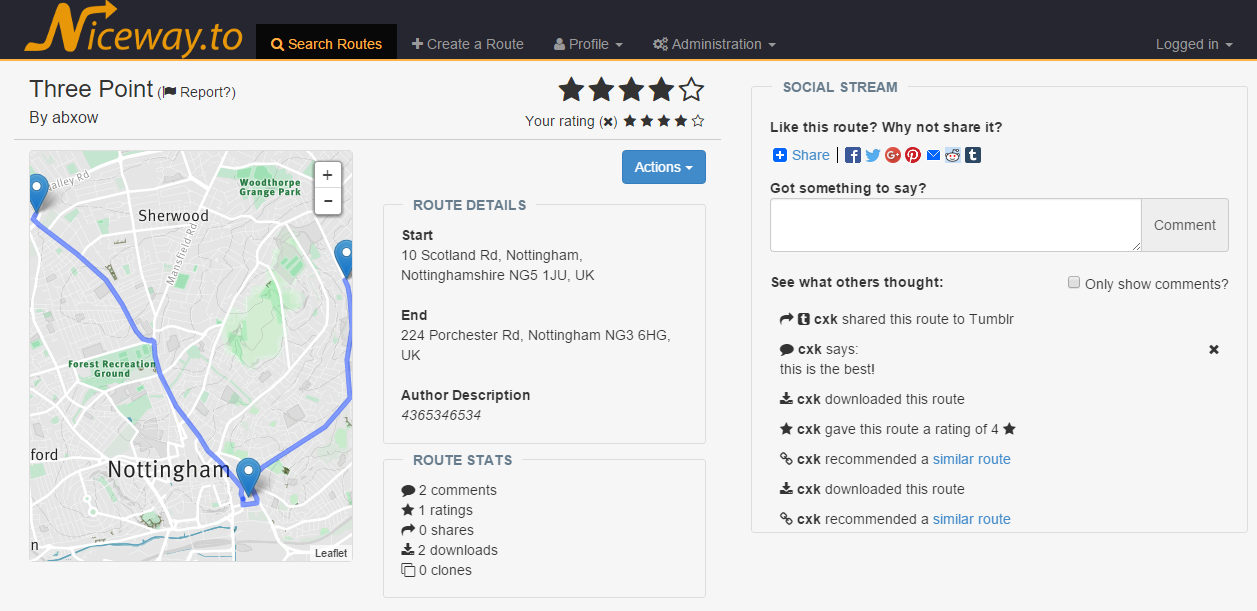
\includegraphics[width=0.9\textwidth]{images/design/detail.png}
	\end{center}
	\vspace{-8mm}
\end{figure}

\noindent
The route detail page was the page used to list all information about one specific route - for this reason, there was a lot of potential for this page to become cluttered. To combat this, the page is clearly divided into two main segments, which are then also further divided. These main sections were the route details on the left, and the route social stream on the right. This clear separation and hierarchical structure to the page made it very easy for users to locate specific information, by slowly narrowing down their search to different areas of the page. \ \\
\ \\
The details section of the page contained a map of the route, key information about it (both administrative information like it's name, and practical information like where it starts), as well as social statistics, like the number of comments and shares (allowing users to see a numeric representation of the popularity of the routes). This meant that users could garner all the information they needed to actually experience the route, as well to see the route they would be following. Being on the left, it is likely users will look at this section first, which means they can quickly determine if they have navigated to the wrong route.\ \\
\ \\
On the right was the social stream, which displayed an amalgamation of all user social interaction with the route. This included comments, shares, downloads, and all other social interactions available. The purpose of this was to give a complete picture of the all interaction with the route, so that users could fully immerse themselves in it, and see what the community thought. It is very prominently displayed, so that more users are likely to notice it, and are more likely to interact with it (a point that my client stressed was extremely important). The social stream was visible both to users that were logged in, and those that weren't. This meant that registered users could easily share their opinions and interact with the route, and non registered users were more convinced to register, so they can could join in with the discussion.

\paragraph{Route Creation Page}\ \\
\begin{figure}[!ht]
	\vspace{-5mm}
	\begin{center}
		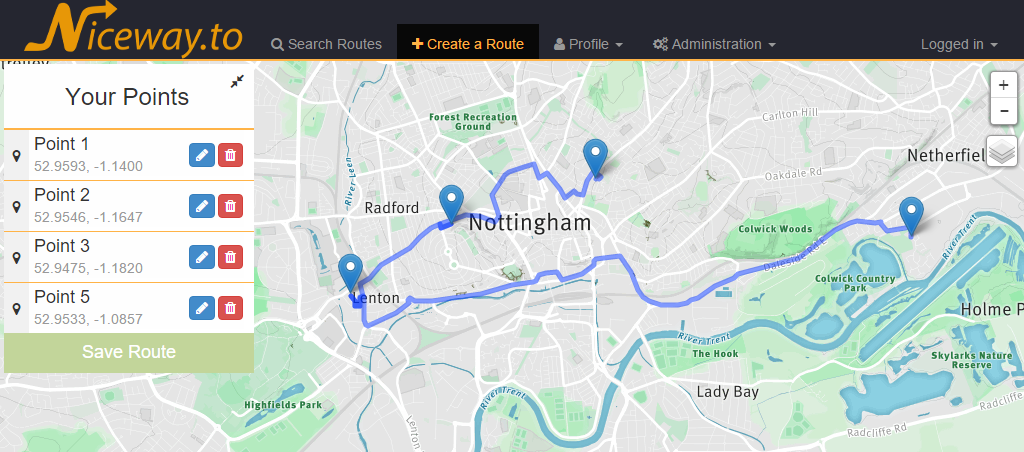
\includegraphics[width=0.99\textwidth]{images/design/create.png}
	\end{center}
	\vspace{-5mm}
\end{figure}

\noindent 
The route creation page was the page that would be used to actually construct and edit routes. It has a very simple interface that consists of a large map and a list of points on that map. This meant that the user could focus on the primary objective of the page, which was the creation of their map, without being distracted by other, useless interface elements. The list on the left served as a tool for users to track what they had done, easily jump to specific points, and update them. This list could also be collapsed, to take up even less space, to further reduce clutter and allow users to see their maps obscured.\ \\
\ \\
To add points, users only had to click on the map, which meant that using the page was very simple and intuitive. As points are added to the map, a route is drawn between them, during which time a popup is displayed so the user is aware of this. The advantage of drawing the map after each point, is that the user can see how their route is forming, and can make adjustments on the fly, rather than getting to the end, generating the route and realising they'd made a huge mistake. \ \\
\ \\
When the user is done with their route, they can hit the save button to bring up a modal window, allowing them to enter in the name and description of the route. Having this in a modal window helps to further eliminate clutter on the page, as it is only displayed when the user specifically requests it.

\newpage 
\paragraph{Profile Page}\ \\

\begin{figure}[!ht]
	\vspace{-5mm}
	\begin{center}
		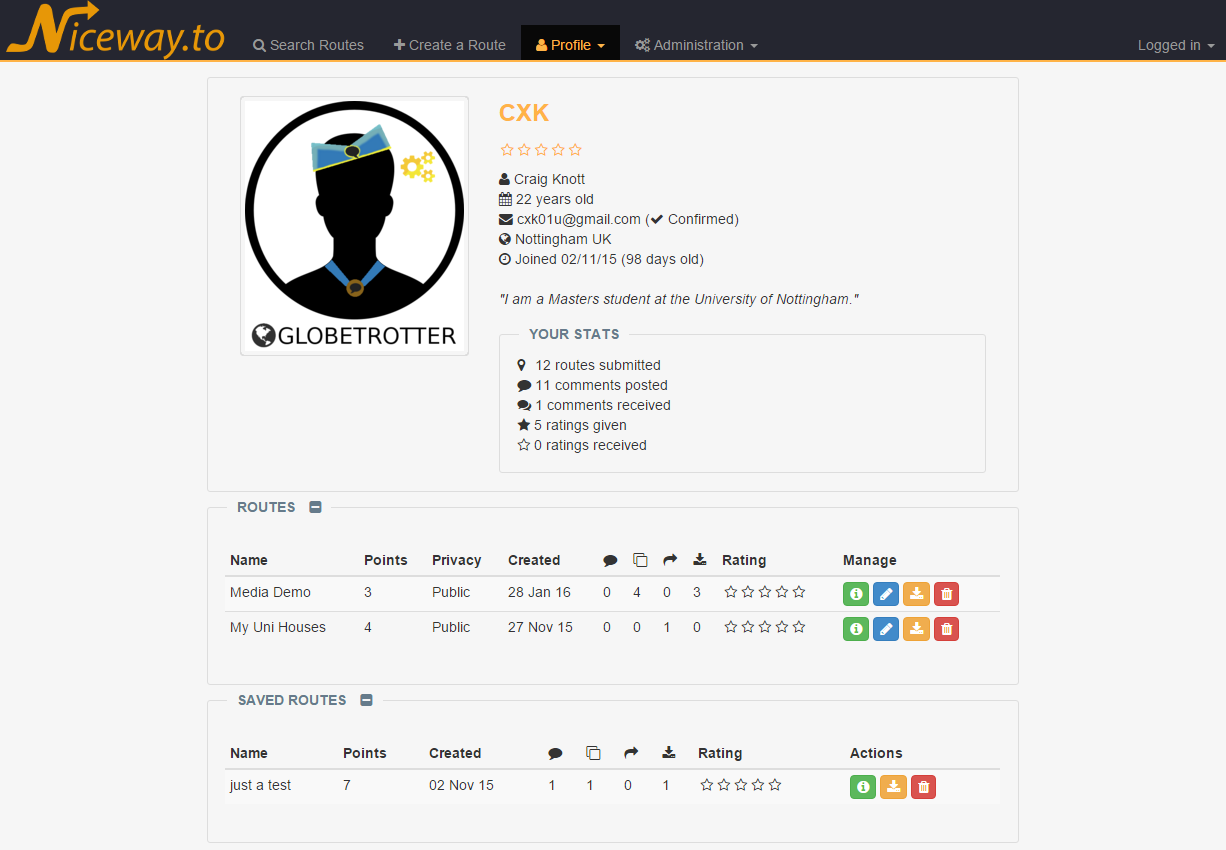
\includegraphics[width=0.95\textwidth]{images/design/profile.png}
	\end{center}
	\vspace{-5mm}
\end{figure}
\noindent 
The final major page for the website was the user profile page, which displays information about a specific user, a list of their routes, and a list of their saved routes. The purpose of this page was to allow users to express themselves to other members of the community, and have somewhere to call ``home''. It displays their public and private details, like their customisation profile image, email account age, and location, and well as statistical information, like the number of comments their routes had received. This meant that other users could quickly build up an idea of what this person is like, and how they interact with the application.\ \\
\ \\
This page also displayed all of the routes that the user had created, which served a different person depending on whether you were viewing your own account page or another user. If viewing your own account page, it served as a central hub to administer and manage all the routes that you had produced, by listing them all, and providing functionality to view them, edit them, or delete them. If viewing another user's profile all of their public routes would be on show. From here, users can view, clone, or download the routes, but not actually make any changes to them. This meant that users could look at the profile of a content producer they enjoyed the work of, and look at other work they had produced. 


\subsubsection{Heuristic Evaluation of the Interface}
In this section, the user interface is evaluated using several key metrics. These include the general purpose usability heuristics identified by Jakob Nielsen\cite{nielsen199510}, and the golden rules of interface design identified by Ben Sschneiderman\cite{shneiderman2005designing}. These have been grouped together with the specific heuristics being labelled in brackets (JN for Jakob, and BS for Ben), a full listing of all the heuristics referenced in this section can be found in appendix \ref{sec:idh}.

\newpage 
\paragraph{Visibility and Feedback (JN1, BS3)}\ \\
Users should always be aware of the impact of their actions. This is why any user interaction will have some visible feedback to the user, which will usually either be the updating of the interface (if something is added or removed), or popup modal windows informing users of what has happened, or what is about to happen.

\paragraph{User should be in full control (JN3, JN7, BS4, BS7, BS8)}\ \\
Users should always be in charge of their experience of the website. This is why they are given full freedom to navigate anywhere within the system (using the navigation bar), and to decide what actions they wish to perform. At no point is the user forced to do anything they have not explicitly requested.

\paragraph{Consistency (JN4, BS1)}\ \\
Consistency is important within a system so users can become accustomed to how things work, and what they mean. This is especially important when users are accessing features for the first time, because they can use their previous knowledge to help them understand the new functionality. This is why colours and icons will be used heavily throughout Niceway.to. Green colours will be used to resemble positive actions (like adding or accepting), and red will be used for negative (deleting or cancelling). Icons for different aspects of the system (like cloning routes, or downloading routes) will be implemented and kept consistent so that users will associate specific icons with specific actions, and they will easily be able to locate and achieve their goals.

\paragraph{Error prevention and Recovery (JN5, JN9, BS5, BS6)}\ \\
It is important that users do not feel punished for making mistakes, and do not get trapped in error states, unable to return. For this reason, extensive error prevention will be implemented, including validation on all forms, confirmations on ``dangerous'' actions, and useful error messages being provided when mistakes are made. The language of these messages is extremely important, as to not make the user feel like they have done something wrong. Instead, users should be instructed on how to resolve the problems they have encountered.

\paragraph{Reduce Cognitive Load (JN6, JN10, BS8)}\ \\
A simplistic design is vital, otherwise users will be encumbered by the sheer quantity of content (it has been shown that humans can only truly cope with between 5 and 9 things at a time\cite{miller1956magical}). If there is too much on the screen at once, users will be confused and unable to focus. This is why only relevant and useful data is displayed to the user, and interfaces are kept as minimalistic as possible. Another way to reduce the cognitive load on the user is to remember data for them. This is the principle applied on the search results page, where the search terms are displayed to the user, which allows them to drop them from their short term memory. 

\paragraph{Match between system and the real world (JN2)}\ \\
The system should use language and imagery that is common and well known, rather than specific to the application. This helps the user's general understanding of the system, as they can relate it to other systems they have used. One example of this in practice is the use of the word ``clone'', for the forking of routes. Forking is a term well known in the field of computer science, but many average users would not understand it, hence this simplification. This is also the reason that icons are used throughout the system, as many users will recognise them and will understand the system better with their inclusion.

\newpage 
\subsection{Internal Design}
As well as the front end, the inner workings of the back end of the system also needed some design. At this point during the project, the Zend framework had been picked as the back end framework (for reasons discussed in section \ref{sec:kid}), which enforces a Model-View-Controller design pattern. The advantages of the MVC framework are that it is simple to understand and use, provides separation of the accessing, processing and display of data, and is extremely modular. The diagram in figure \ref{fig:mvc} shows the interaction that users would have with the front end and back end of the system. It begins with a user on some web-browser making a request for a specific page. The browser then talks to the Controller (firstly the base controller, and then the specific controller for that page), which usually requests some data from the database. This access is abstracted, and is facilitated through the Model and various factories of the system, which actually access the data, and returns the results as a PHP object. The controller then passes this data on the View, which displays the user interface and is served to the client for them to interact with.

\begin{figure}[!ht]
	\begin{center}
		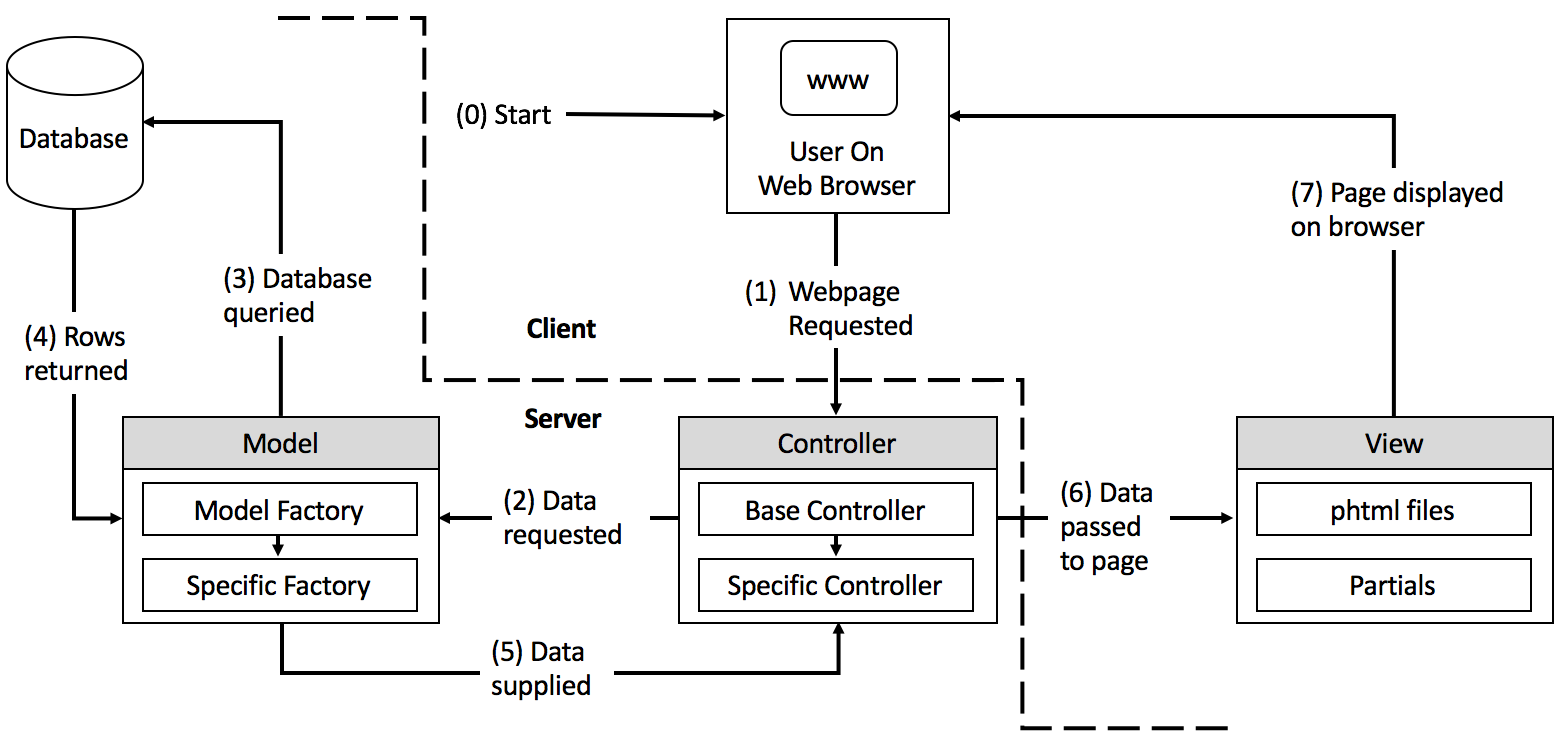
\includegraphics[width=0.9\textwidth]{images/design/internal.png}
	\end{center}
	\vspace{-6mm}
	\caption{The internal design of Niceway.to}
	\label{fig:mvc}
\end{figure}

